\begin{exercise}
 Show that $f_i$ is an involution without a fixed point.
 That is, $f(f(x)) = x$ and $f(x) \ne x$ for all $x \in \{0,1\}^d$.
\end{exercise}

\begin{proof}
According to definition, $f_i(x)$ is x with $i^{th}$ position flipped, so $f_i(x) \neq x$. And $f_i(f_i(x))$ is x with $i^{th}$
position flipped twice, which goes back to x, so $f_i(f_i(x)) = x$.Therefore, $f_i$ is an involution without a fixed point.\\
\end{proof}

Let $S \subseteq \{0,1\}^d$. We define  $f_i(S)$ as the set arising from applying
$f_i$ to every element of $S$. Formally,
\begin{align*}
f_i(S) := \{ f_i(x) \ | \ x \in S \} \ .
\end{align*}
Given a set $S \subseteq \{0,1\}^d$, we call an index $i \in [n]$ {\em active} for $S$
if $f_i(S) \ne S$. 
\begin{exercise}
Let $d=3$ and $S = \{000, 100\}$. Which of the indices $1,2,3$ are active?
\end{exercise}

\begin{proof}
Let least significant digit be the 1'st position.\\
\[f_1(S) = \{001,101\} \neq S\]
\[f_2(S) = \{010,110\} \neq S\]
\[f_3(S) = \{100,000\} = S\]
So 1 and 2 are active.
\end{proof}

\begin{exercise}
 Show that $f$ is an involution. That is, $f(f(S)) = S$. Furthermore, show that
 the only fixed points of $f$ are $\emptyset$ and $\{0,1\}^d$.
\end{exercise} 

\begin{proof}
\[\forall x \in S, f(f(x)) = x \Rightarrow f(f(S))=S\]
If $S= \emptyset$, $f(S)=S$.If there is at least one element in S and $f(S)=S$. We call the element as $x_{0\ldots 00}$. Since $f(S) = S$, $f_1(x) \in S$, which is named as $x_{0\ldots 01}$.Then, $f_2(x), f_2(x_1) \in S$, which is named as $x_{0\ldots 10} \: and\: x_{0\ldots 11}$.Similarly, we can deduce that $x_{0\ldots 00},x_{0\ldots01},x_{0\ldots 10}\ldots ,x_{1\ldots 11} \in S$, which means $S = \{0,1\}^d$. So $f(S)=S \Rightarrow S=\emptyset \: or\: \{0,1\}^d$. That is to say that the only fixed points of $f$ are $\emptyset$ and $\{0,1\}^d$.
\begin{center}
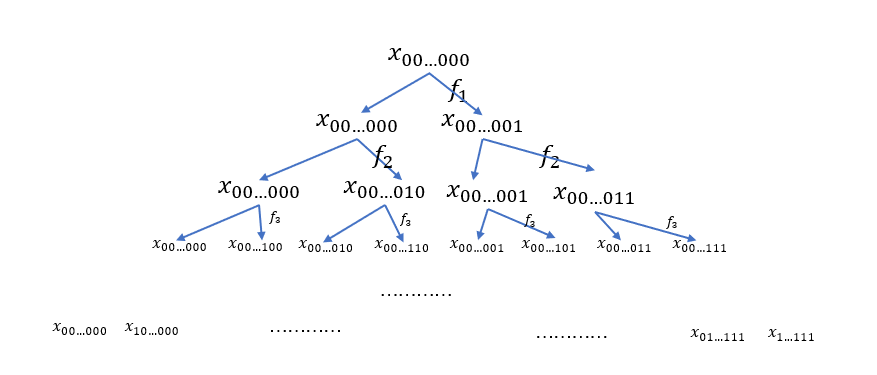
\includegraphics[scale=0.8]{10.png} 
\end{center}
\end{proof}

\begin{exercise}
   Let $\mathcal{S} = { \{0,1\}^d \choose k }$. This is a set of sets, and each set $S \in \mathcal{S}$
   consists of exactly $k$ strings from $\{0,1\}^d$. Prove the following statements: 
   \begin{enumerate}
   \item $f$ is a bijection from $\mathcal{S}$ to $\mathcal{S}$.
   \item For $1 \leq k \leq 2^d-1$, this bijection is an involution
   without fixed points.
   \item $|\mathcal{S}|$ is even for $1 \leq k \leq 2^d-1$.
   \end{enumerate}
\end{exercise}

\begin{proof}
1. $\forall S \in \mathcal{S}$, f(S) also consists of k strings, which means $f(S) \in \mathcal{S}$. So f is a bijection from $\mathcal{S}$ to $\mathcal{S}$.
\end{proof}

\begin{proof}
2. According to Exercise 4.10, For $1 \leq k \leq 2^d-1$, which means $S \neq \emptyset \: and\: S \neq \{0,1\}^d$, $f(S) \neq S$.So f is an bijection without fixed point.
\end{proof}

\begin{proof}
3. Since $f(S)\neq S$and $f(f(S))=S$, we say every S can be "married" with f(S).Thus,$|\mathcal{S}|$ is even for $1 \leq k \leq 2^d-1$.
\end{proof}

